\documentclass[11pt,spanish]{article}

% Paquetes
\usepackage{amstext}
\usepackage{amssymb}
\usepackage{amsmath}
\usepackage{babel}
    \addto\shorthandsspanish{\spanishdeactivate{~<>}}
    \decimalpoint
\usepackage[style=iso]{datetime2}
\usepackage{fancyhdr}
\usepackage{float}
\usepackage[T1]{fontenc}
\usepackage[a4paper]{geometry}
    \geometry{verbose,tmargin=3cm,bmargin=2cm,lmargin=2.5cm,rmargin=2.5cm}
\usepackage{graphicx}
\usepackage{hyperref}
\usepackage[utf8]{inputenc}
\usepackage{lastpage}
\usepackage{mathptmx}
\usepackage{tasks}
\usepackage{units}
\usepackage{siunitx}

% dibujos 

\usepackage{tikz}
\usepackage{tikz-dimline}
\usetikzlibrary{calc}
% \usetikzlibrary{math}
\usetikzlibrary{arrows.meta}
\usetikzlibrary{snakes}
\usetikzlibrary{decorations}
\usetikzlibrary{decorations.pathmorphing}
\usetikzlibrary{patterns}

% tipo de fuente 
\usepackage{lmodern}

\pagestyle{fancy}
\lfoot{\small DF, FCEyN, UBA}
\cfoot{\tiny Actualizado el {\today} a las {\DTMcurrenttime}}
\rfoot{\small Pág. {\thepage} de \pageref{LastPage}}

\begin{document}

% Título
    \begin{center}
    \textsc{\large Física 2 (Física) - Cátedra Diana Skigin}
    \par\end{center}{\large \par}
    
    \begin{center}
    \textsc{\large Segundo Cuatrimestre de 2021}
    \par\end{center}{\large \par}
    
    \begin{center}
    \textsc{\large Guía 7: Propagación de la luz}
    \par\end{center}{\large \par}

% Comienzo 
\begin{enumerate}

\section*{Principio de Fermat}

% Ejercicio 1

    \item Considere un rayo que parte del punto $A=(0,1,0)$, se refleja en un
    espejo plano situado en el plano $xz$, y finalmente pasa por el punto
    $B=(4,3,0)$. Emplee el principio de Fermat para responder las siguientes
    preguntas. Interprete físicamente los resultados.
    \begin{enumerate}
        \item ¿En qué punto sobre el plano del espejo se produce la reflexión?
        \item ¿Cuánto valen los ángulos de incidencia y reflexión?
        \item Un rayo directo entre $A$ y $B$ recorre un menor camino óptico que
        el hallado en los ìtems \textit{a} y \textit{b}, ¿es esto contradictorio?
    \end{enumerate}

% Ejercicio 2

    \item A partir del principio de Fermat, deduzca la ley de Ibn Sahl-Snell
    para la refracción de la luz entre dos medios con índices de refracción
    $n_{1}$ y $n_{2}$, separados por una superficie plana.

% Ejercicio 3

    \item Considere un espejo elíptico con focos $A$ y $B$. En $A$ hay una
    fuente puntual. Uno de los rayos emitidos por la fuente impacta en el punto
    $C$ y se refleja hacia el otro foco $B$.
    
    \begin{enumerate}
        \item Muestre que el camino óptico del rayo mencionado es estacionario
        en la elipse.
        
        \item Considere ahora que se reemplaza la elipse por un espejo plano o
        uno esférico, tangentes a la elipse en el punto $C$. Determine
        cualitativamente si el camino óptico del rayo que impacta en $C$ es
        máximo, mínimo o estacionario cuando se refleja en cada uno de los
        espejos.
    \end{enumerate}

    \begin{figure}[H]
        \centering
        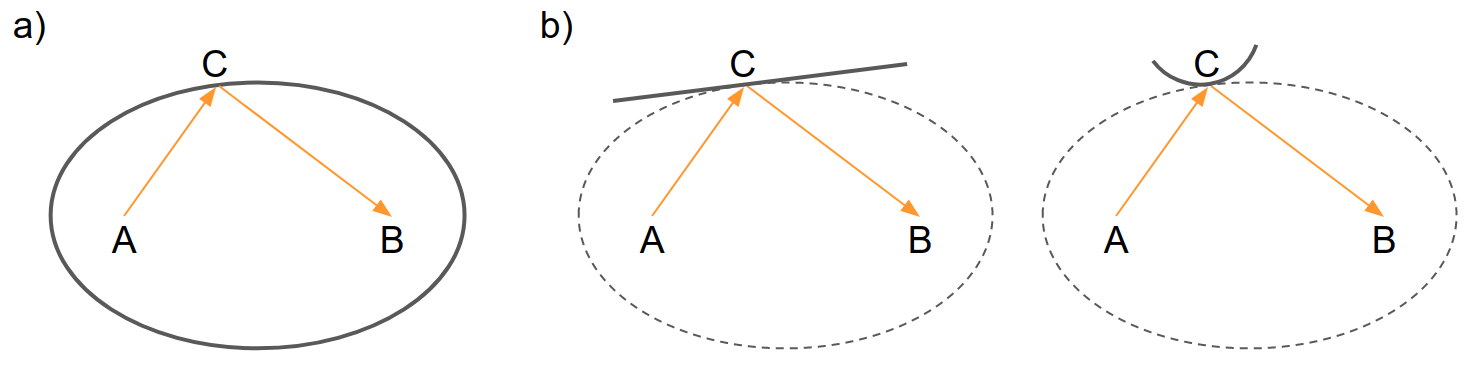
\includegraphics[width=12cm]{figs/eliptico.png}
    \end{figure}


\section*{Reflexión y refracción}

% Ejercicio 4

    \item 
    \begin{enumerate}
    	\item Un rayo de luz llega a una interfaz aire-líquido con una
        inclinación respecto a la normal de \ang{55}. El rayo refractado se
        transmite formando un ángulo igual a \ang{40}. ¿Cuál es el índice de
        refracción del líquido?
    	
    	\item Un haz de luz incide desde aire sobre una lámina de vidrio de
        índice de refracción desconocido y espesor $d$. Al otro lado del vidrio
        hay agua ($n_\text{agua}= 1.333$). El ángulo de incidencia en la
        interfaz aire-vidrio es \ang{30}. Calcule el ángulo que el rayo
        refractado forma con la normal a la superficie en el agua.
    	
    	\item Un rayo de luz se propaga en un medio cuyo índice de refracción
        es $n_1=2$. Dicho rayo incide sobre otro medio de índice de refracción
        $n_2=1.5$, formando un ángulo de \ang{30} respecto a la normal a la
        superficie de separación. Calcule el ángulo que forma el rayo
        transmitido con la normal a la superficie. ¿Con qué inclinación mínima
        debería incidir el rayo para que no haya transmisión?
    \end{enumerate}

% Ejercicio 5

    \item Considere un rayo que incide sobre una lámina de caras paralelas de
    espesor $d$ inmersa en un medio único.
    \begin{enumerate}

        \item Demuestre que el rayo incidente no se desvía al atravesarla (es
        decir, que el rayo emergente B tiene la misma inclinación que el rayo
        incidente A).
        
        \item Calcule el desplazamiento lateral $\Delta$ en términos del espesor
        y el índice de refracción de la lámina.

        \item Demuestre que el rayo que se refleja en la primera cara y el que
        emerge luego de reflejarse en la segunda son paralelos.
        
        \item Si el medio exterior es único, ¿existe algún ángulo de incidencia
        tal que produzca reflexión total en la segunda cara?

    \end{enumerate}
    
    \begin{figure}[H]
        \centering{}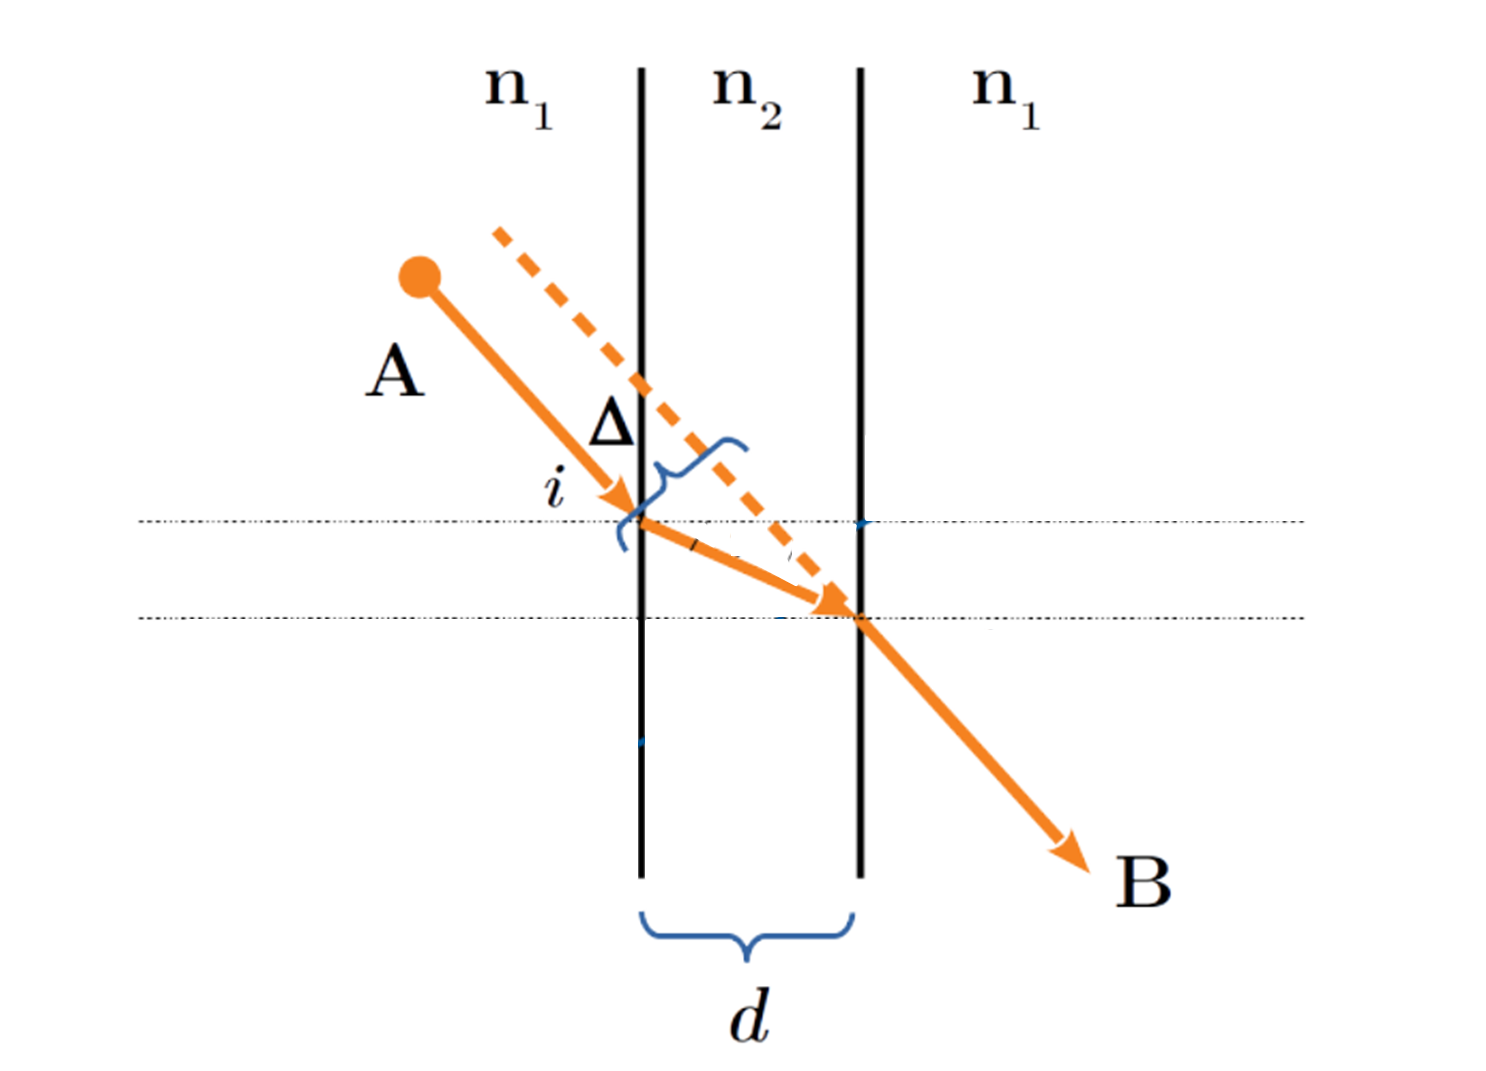
\includegraphics[clip,scale=0.15]{figs/a-000.png}
    \end{figure}

% Ejercicio 6

    \item Un rayo incide con ángulo $\phi$ sobre la superficie horizontal de
    un cubo de material transparente, de índice $n$, inmerso en aire.
    \begin{figure}[H]
        \centering{}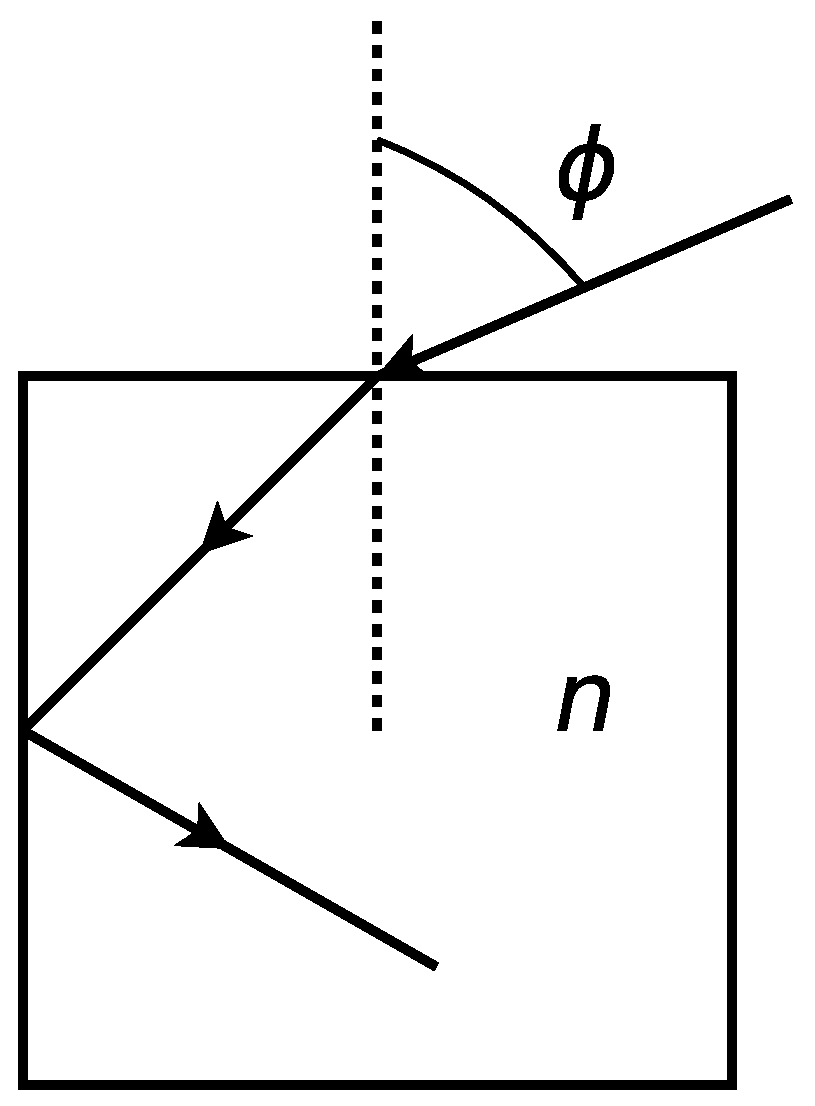
\includegraphics[clip,scale=0.25]{figs/ej3-5}
    \end{figure}
    
    \begin{enumerate}
        \item ¿Para qué valores de $\phi$ hay reflexión total en la cara
        vertical?
        
        \item Si $\phi=60^{\circ}$, ¿cuál es el máximo $n$ para que no haya
        reflexión total en la cara vertical? ¿Se puede reflejar totalmente en
        la cara superior?
    \end{enumerate}

% Ejercicio 7

    \item Los índices de refracción de cierta clase de vidrio para las
    longitudes de onda correspondientes al rojo ($\lambda_\text{rojo} \sim 665$
    nm) y violeta ($\lambda_\text{azul} \sim 470$ nm) valen $1.51$ y $1.53$,
    respectivamente.
    
    \begin{enumerate}
        \item Halle los ángulos límite de reflexión total para rayos de luz que
        incidan en la superficie de separación vidrio-aire, para esas longitudes
        de onda.
    
        \item ¿Qué ocurre si un rayo de luz blanca incide formando un ángulo de
        41$^{\circ}$ sobre dicha superficie? \textbf{Sugerencia:} Extrapole el
        índice de refracción para longitudes de onda visibles a partir de la
        información para las longitudes extremas del mismo, y determine el
        comportamiento en función de la longitud de onda.
    \end{enumerate}

\section*{Prismas}    
    
% Ejercicio 8
    
    \item 
    \begin{enumerate}
        \item Calcule analíticamente el ángulo de desviación mínima del prisma.
        Justifique por qué este valor es único. Haga un gráfico cualitativo
        de la desviación como función del ángulo de incidencia.

        \item Calcule la desviación mínima para prismas delgados, en función de
        los datos constructivos.

        \item Si el prisma es delgado y el ángulo de incidencia es pequeño,
        calcule la desviación.
    \end{enumerate}

% Ejercicio 9

    \item 
    \begin{enumerate}
        \item En un vidrio óptico común se propaga un haz de luz blanca, ¿qué
        componente viaja más rápido: la roja o la violeta?

        \item ¿Para cuál de ambos colores será mayor la desviación en un prisma?
        ¿Qué puede decir del ángulo de desviación mínima? Justifique sus
        respuestas.
    \end{enumerate}

% Ejercicio 10

    \item Dado un prisma de vidrio crown\footnote{El vidrio crown se caracteriza
    por tener muy baja dispersión cromática.} de ángulo $\alpha=4^{\circ}$
    calcular, para las líneas de absorción de Fraunhofer \textbf{F}
    ($\lambda_\text{F} = 486.134 $ nm), \textbf{D} ($\lambda_\text{D} = 589.293
    $ nm) y \textbf{C} ($\lambda_\text{C} = 656.281$ nm), las desviaciones de
    rayos que inciden casi perpendicularmente. Los respectivos índices de
    refracción son: $n_\text{F}=1.513$; $n_\text{D}=1.508$ y $n_\text{C}=1.504$.
    
\end{enumerate}

\end{document}

